\documentclass[english,12pt,twoside,a4paper]{report}
	\usepackage[ngerman,english]{babel}		% Language specification
	\usepackage{varioref}		% Better references but possibly unstable
	\usepackage[utf8]{inputenc}
	\usepackage[T1]{fontenc}		% Required to output umlauts in a PDF
	\usepackage{pslatex}
	\usepackage{amsmath}
	\usepackage{multirow}
	\usepackage{ellipsis}
	\usepackage{textcomp}
	\usepackage{longtable}
	\usepackage{rotating}
	\usepackage[section]{placeins}

	\usepackage[font=small,labelfont=bf]{caption}		% Customize caption aesthetics
	\usepackage[font=small]{subcaption}

	\usepackage{xcolor}		% Highlighting
	\usepackage{tcolorbox}		% Fancy colored boxes
	\usepackage{soul}

	\usepackage[tracking=true]{microtype} % required to change character spacing

	\usepackage{listings}		% Insert programming code
	\usepackage{graphicx}		% Required to insert images
	\usepackage[space]{grffile}		% Insert images baring a filename which contains spaces
	\usepackage{float}		% Forcefully set the location of an object

	\usepackage[style=numeric,backend=biber]{biblatex}
	\usepackage[bookmarks]{hyperref}	% Clickable references

	\usepackage[nodayofweek]{datetime}	% Flexible date specification
	\newcommand{\leadingzero}[1]{\ifnum#1<10 0\the#1\else\the#1\fi}
	\newcommand{\todayddmmyyyy}{\leadingzero{\day}.\leadingzero{\month}.\the\year}
	\newcommand{\mathcolorbox}[2]{\colorbox{#1}{$\displaystyle #2$}}

	\usepackage{geometry}
	\usepackage{scrextend}		% Arbitrary indentation

	\usepackage{color}

	\addbibresource{../literature.bib}

	\makeatletter
	\makeatother

	\pagestyle{headings}
	\oddsidemargin0.8cm		% Left spacing for pages with an uneven number only relevant for \twoside
	\evensidemargin0.2cm		% Left spacing for pages with an even number only relevant for \twoside
	\topmargin0.5cm		% Top spacing
	\textheight21cm		% Height of the text on a page
	\textwidth15cm		% Width of the text on a page
	\renewcommand{\topfraction}{0.75}		% Fraction of flowing boxes at the beginning of a page
	\renewcommand{\bottomfraction}{0.75}		% Fraction of flowing boxes at the end of a page
	\renewcommand{\sectionautorefname}{\ifnum\spacefactor>1000 Section\else section\fi}		% Capitalize 'section' if used after some spacing
	\parskip1ex  plus1ex minus0.5ex		% Spacing between paragraphs
	\parindent0em		% Indentation of the first line of a paragraph
	\newcommand{\clearemptydoublepage}{\newpage{\pagestyle{empty}\cleardoublepage}}

	\def\permille{\ensuremath{{}^\text{o}\mkern-5mu/\mkern-3mu_\text{oo}}}

	\title{Optimization of Particle Identification}
	\author{\href{mailto:gordian.edenhofer@gmail.com}{Gordian Edenhofer}}
	\date{29. June 2018}

\begin{document}

\selectlanguage{english}

\pagenumbering{Roman}
%\maketitle
\thispagestyle{empty}
\begin{center}
	\begin{LARGE}
		{
			\bf
			\hspace*{1cm} Optimization of Particle Identification \\ [0.3cm]
		}
	\end{LARGE}
	\vspace{0.5cm}
	%
	\begin{figure}[htbp]
		\begin{center}
			\hspace*{1cm}
			
\includegraphics[height=4cm]{pics/lmu3.pdf}
		\end{center}
		%\label{fig-lmulogo}
	\end{figure}

	\vspace{1.0cm}
	\begin{large}
		\hspace*{1cm}Bachelor thesis at the faculty of physics \\
		\hspace*{1cm}of the \\
		\hspace*{1cm}Ludwig-Maximilians-Universität München \\ [2.5cm]
		\hspace*{1cm}handed in by \\
		{\bf
		\hspace*{1cm}Gordian Edenhofer \\ }
		\hspace*{1cm}born in Frankfurt am Main on the \formatdate{13}{07}{1997} \\ [0.5cm]
		%\hspace*{1cm}\today
		\hspace*{1cm}Munich, the \formatdate{28}{06}{2018}
	\end{large}
\end{center}

\clearpage
\thispagestyle{empty}
\mbox{ }
\setcounter{page}{0}
\clearpage
\thispagestyle{empty}
\begin{center}
	\selectlanguage{ngerman}

	\begin{LARGE}
		{
		\bf
		\hspace*{1cm} Optimierung der Teilchenidentifizierung \\ [0.3cm]
		}
	\end{LARGE}
	\vspace{0.5cm}
	%
	\begin{figure}[htbp]
		\begin{center}
			\hspace*{1cm}
			
\includegraphics[height=4cm]{{{../res/LMU logo}}}
		\end{center}
		%\label{fig-lmulogo}
	\end{figure}

	\vspace{1.0cm}
	\begin{large}
		\hspace*{1cm}Bachelorarbeit an der Fakultät für Physik \\
		\hspace*{1cm}der \\
		\hspace*{1cm}Ludwig-Maximilians-Universität~München \\ [2.5cm]

		\hspace*{1cm}vorgelegt von \\
		{
		\bf
		\hspace*{1cm}Gordian~Edenhofer \\
		}
		\hspace*{1cm}geboren in Frankfurt am Main am \datengerman\formatdate{13}{07}{1997} \\ [0.5cm]

		\hspace*{1cm}München, den \datengerman\formatdate{29}{06}{2018} \\ [0.5cm]

		\hspace*{1cm}Betreuer: \\
		{
		\bf
		\hspace*{1cm}Prof.~Dr.~Thomas~Kuhr
		}
	\end{large}
\end{center}

\clearpage
\thispagestyle{empty}
\mbox{ }
\setcounter{page}{0}
\clearpage
\chapter*{Abstract}

This study aims at evaluating further particle identification approaches.
At first the goodness of the detector variables is measured. Flaws are outlined and possible causes are evaluated. Afterwards further techniques are discussed which combine the detector variables in a new way.

A Bayesian approach to particle identification is discussed. It aims at producing probabilities of a track belonging to a particle species in dependance of the received signal. The process of obtaining the conditional probabilities is described in greater detail. In addition, some extensions to the Bayesian approach are presented and evaluated. Flaws and benefits are compared using a generic decay.

Lastly, a neural network is used to label particle tracks. For a simple network, different methods to adapt the weights and various input forms are evaluated. Hereby, tools from machine learning and statistics are discussed and their application is outlined. In the end the accuracy of the network on a generic decay is determined.

\clearpage

\tableofcontents
\cleardoublepage

\pagenumbering{arabic}

\chapter{Introduction}
\label{chap:introduction}

Since the dawn of physics one of the most fundamental question has been to find the most elemental constituents of matter. In this regard the standard model has proven to be extremely useful. It postulates six quark species \{up, down, strange, charm, bottom, top\}, three charged kinds of leptons \{electron, muon, tau\}, a neutral neutrino for every charged lepton specie and four species of gauge bosons \{photon, $W$, $Z$, gluon\} as well as the Higgs boson $H$. Besides its achievement in describing the very basic principals of interactions and its experimental predictions being very precise, there emerged significant flaws; namely the high energy limit, matter \& anti-matter asymmetry and the existence of dark matter and dark energy.

The Belle~\RN{2} experiment was designed to aid in the search for new physics phenomena with a massive volume of data in the flavour sector. The violation of $CP$-symmetry has already been observed at the predecessor experiment Belle. However, analysis of rare decays with only small corrections to the Standard Model are hard to spot and require more statistics. At the hardware frontier the detector and accelerator system was updated. The software side required adaption as well to cope with the massive amount of data.

In order to spot such small deviations in such large sets of data, a reliable particle identification is a fundamental requirement. Its role is to assign particle species labels to tracks which are identified by the detector system. By doing so, it allows further analysis of events to focus on the particles relevant to them.

\chapter{Belle~\RN{2}}
\label{chap:belle2_experiment}

\section{Experiment}
\label{sec:experimental}

The Belle~\RN{2} experiment is performed at the SuperKEKB accelerator located in Tsukuba, Japan. It is mainly designed to study B mesons.
In the experiment, asymmetric electron- positron-beams are collided with a center of mass energy of $\sqrt{s} = 10.58 \mathrm{~GeV}$, exactly on the $\Upsilon (4S)$ resonance. The two beams, positrons at $4 \mathrm{~GeV}$ and electrons at $7 \mathrm{~GeV}$, are focussed to a narrow crossing section. The additional boost in one direction is used to measure the $B$ meson lifetimes.

In comparison to the predecessor experiment Belle, the integrated luminosity will be $50~{ab}^{-1}$ and hence $50$ times higher. The instantaneous luminosity will be $8 \cdot 10^{35} \mathrm{cm}^{-2} \mathrm{s}^{-1}$, which is a $40$-fold increase.

\section{Detector system}
\label{sec:detector_system}

\subsection{Overview}
\label{sec:detector_system_overview}

The Belle~\RN{2} detector system~\cite{Abe:2010gxa,Pulvermacher:SuperKEKBDetectorComponents,Pulvermacher:AnalysisSoftware} is a composition of multiple detectors, each measuring a subset of a particle's properties. Its design is depicted in~\autoref{fig:belle2_detector_design_white_paper}.
The inner three detectors -- \textbf{P}i\textbf{X}el \textbf{D}etector (PXD), \textbf{S}ilicon \textbf{V}ertex \textbf{D}etector (SVD) and \textbf{C}entral \textbf{D}rift \textbf{C}hamber (CDC) -- record the position of traversing charged particles. Hence they are also called tracking detectors. They are located in a homogeneous magnetic field of $1.5~\mathrm{T}$.
The innermost detector is the PXD. Together with the SVD which surrounds the PXD, it is used to reconstruct decay vertices and identify tracks belonging to particles with low-momenta.
The CDC measures the momentum and charge of particles via their curvature in the magnetic field.
Next, the \textbf{T}ime \textbf{O}f \textbf{P}ropagation counter (TOP) (`Barrel~PID') and the \textbf{A}erogel \textbf{R}ing-\textbf{I}maging \textbf{CH}erenkov (ARICH) counter (`Endcap~PID') are used to identify charged particles via their emission of Cherenkov radiation in the detector. However, there is no such installation for the backwards-facing endcap of the detector due to the asymmetric beams.
The \textbf{E}lectromagnetic \textbf{C}a\textbf{L}orimeter (ECL) identifies photons and electrons.
The outermost detector called $\boldsymbol{K}^0_{\boldsymbol{L}}$/$\boldsymbol{\mu}$ (KLM) is used to identify kaons and muons\footnotemark.
\footnotetext{If not specifically stated otherwise, the charge conjugate of a particle is implied.}

\begin{figure}[ht]
	\centering
	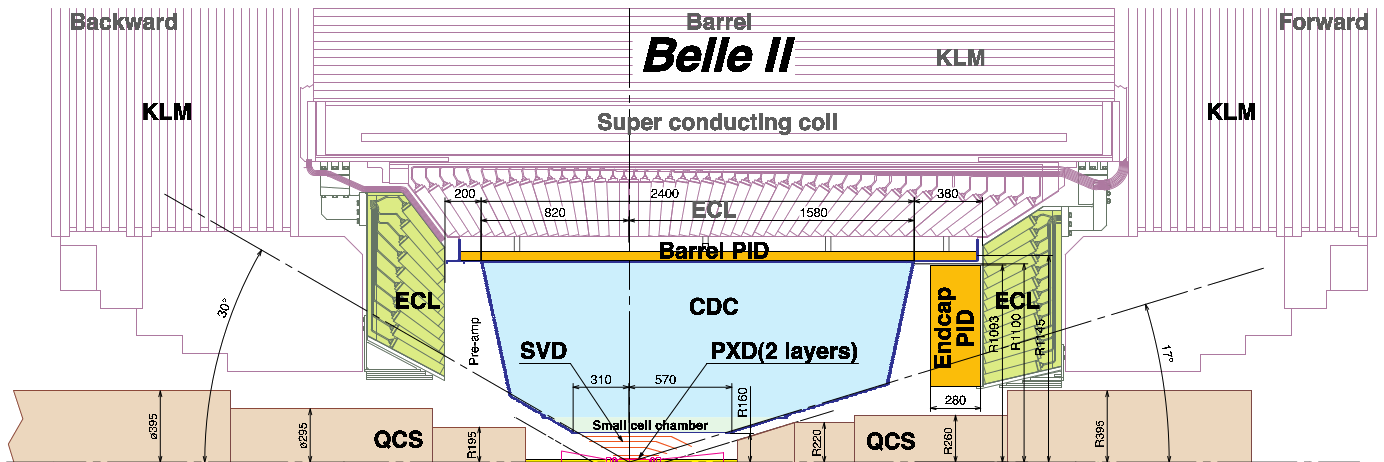
\includegraphics[width=\textwidth,height=0.6\textheight,keepaspectratio]{{{../res/Belle 2 detector design white paper (truncated)}}}
	\caption{Side view of the upper half of the Belle~\RN{2} detector. Adapted from~\cite{Abe:2010gxa}.}
	\label{fig:belle2_detector_design_white_paper}
\end{figure}

\subsection{Silicon detectors}
\label{sec:detector_system_silicon_detectors}

The PXD and SVD consist of tiny doped silicon chips which yield the location of electron-holes created by particles passing through it. The PXD detector uses small pixels while the SVD detector uses strips of detector material. Therefore, the PXD detector is able to further differentiate multiple simultaneous tracks while the SVD allows for a faster readout and is less prone to noise.

\subsection{Central drift chamber}
\label{sec:detector_system_tracking_detectors}

The CDC, which surrounds the PXD and SVD, consists of a collection of field wires and sense wires located in a volume filled with gas. The sense wires are used to measure the current produced by electromagnetic showers. The latter is caused by particles passing through the gas. The wires are close to being parallel to the beampipe but have a slight twist. This allows the detector to not only have an excellent estimation of the transverse distance to the beam pipe but also provides information about the longitudinal position.

\subsection{Barrel and endcap PID}
\label{sec:detector_system_barrel_and_endcap_pid}

The Cherenkov effect is used to measure the velocity of particles in the TOP and ARICH detector. Charged particles which travel faster than the speed of light in the medium -- Quartz in case of the TOP detector and aerogel for the ARICH detector -- produce light. The velocity can be calculated by measuring the time of propagation and the angle of the emitted light.

\subsection{Electromagnetic calorimeter}
\label{sec:detector_system_electromagnetic_calorimeter}

The main purpose of the ECL detector is to determine the energy of photons and electrons. Both particle species excite the medium and create electromagnetic showers. The light of the de-excitation can subsequently be measured.

\subsection{$\boldsymbol{K}^0_{\boldsymbol{L}}$/$\boldsymbol{\mu}$ detector}
\label{sec:detector_system_k0lmu}

Last but not least, the KLM detector identifies kaons and muons which have passed through the previous layers of the system. When traversing this detector, the particles pass through plates serving as electrodes separated by layers of gas in between them. Ionized particles are accelerated in this field and subsequently produce a spark picked up by the detector via measuring the drop in voltage.

\section{Interaction with matter}
\label{sec:interaction_with_matter}

\subsection{Charged particle interaction}
\label{sec:interaction_with_matter}

Particles with non-zero charge mainly interact with the medium electromagnetically. In general, an interaction occurs either by scattering in the electric field of the atom, polarization of the medium, ionization or excitation. Besides, hadrons may scattering at the atom itself. Particles and their anti-particles additionally have the ability to annihilate.

The polarization of the medium causes Cherenkov radiation to be emitted. At velocities below the speed of light in the medium ($v < c/n$), only boundaries of the particle's velocity may be determined. However, at $v > c/n$ the Cherenkov effect can be observed. The effect occurs due to the information about the charge of the traversing particle not reaching the medium in front of it soon enough. Hence, the medium behind the particle is already aligned with the electric field while the medium in front is not. The result is an electromagnetic wave. The angle between the normal vector of the wave and the track of the particle is given by
\begin{equation}
	\cos(\Theta_{c}) = \frac{1}{v/c \cdot n} = \frac{1}{\beta \cdot n}
	\mathrm{.}
\end{equation}
This is the effect which the TOP and ARICH detectors exploit.

Particles with low energy traveling through a medium interact predominantly with atomic electrons. The average energy loss of a particle is described by the Bethe-Bloch formula. It is given by $\left< \mathrm{d}E/\mathrm{d}x \right> \propto 1/{\beta^2}$ for velocities of up to about $90\%$ of the speed of light and is minimal at $\beta \gamma \approx 4$. It describes the momentum dependency of the average energy loss. However, the actual shape of $\mathrm{d}E/\mathrm{d}x$ is modelled by the Landau distribution. Note that the initial assumptions needed for this formula are not met for electrons. This is because both participants of the interaction belong to the same species and have identical masses.
A $\mathrm{d}E/\mathrm{d}x$-measurement is performed at the silicon detectors and the CDC.

The interaction with the electromagnetic field of the nucleus is the dominant cause for the energy loss of high-energy particles. Energy is radiated away via so called Bremsstrahlung. The leftover energy decreases exponentially with the distance traversed and is inversely proportional to the square root of the mass. Therefore it is mainly important for particles with a low mass, e.g., electrons. The radiation due to this effect is mainly measured by the ECL.

\subsection{Particle identification}
\label{sec:particle_identification}

At Belle~\RN{2} the detector system differentiates among six long living particle species $K, \pi, e, \mu, p \text{ and } \hbox{deuteron}$.

The $\mathrm{d}E/\mathrm{d}x$-measurement from the silicon detectors and the CDC are one of the most useful measurements. \autoref{fig:de_dx_for_SVD} showcases this for one of the tracking detectors for momenta below $1 \mathrm{~GeV/c}$. Distinct patterns may be observed for various particle species below this momentum threshold.
New tracks can now be assigned a likelihood of producing the measured detector signal given they belonging to a certain particle species. This is done by postulating a hypothesis for the loss of energy for each such species.

ARICH, TOP and CDC furthermore extend the identification and are able to differentiate among $K, \pi, p \text{ and } \hbox{deuteron}$ but also contribute to $e$ and $\mu$ identification. They provide likelihoods for each signal given a particle hypothesis.

Further out the ECL detector provides a good separation of electrons from other charged particles above $1 \mathrm{~GeV/c}$. It is able to do so via measuring $E/p$ of the shower. The detector response is provided by estimating the degree of agreement for different particle hypothesis with the signal. An exemplary $E/p$ curve is shown in \autoref{fig:e_p_for_ECL}. It demonstrates the observable difference for electrons compared to other particle species but also shows that no clear separation of pions and muons is possible.

The KLM detector provides a good separation between muons and non-muons and contributes to the discrimination in the form of different likelihoods as well.

\begin{figure}[ht]
	\centering
	\subcaptionbox{$\mathrm{d}E/\mathrm{d}x$\label{fig:de_dx_for_SVD}}{
		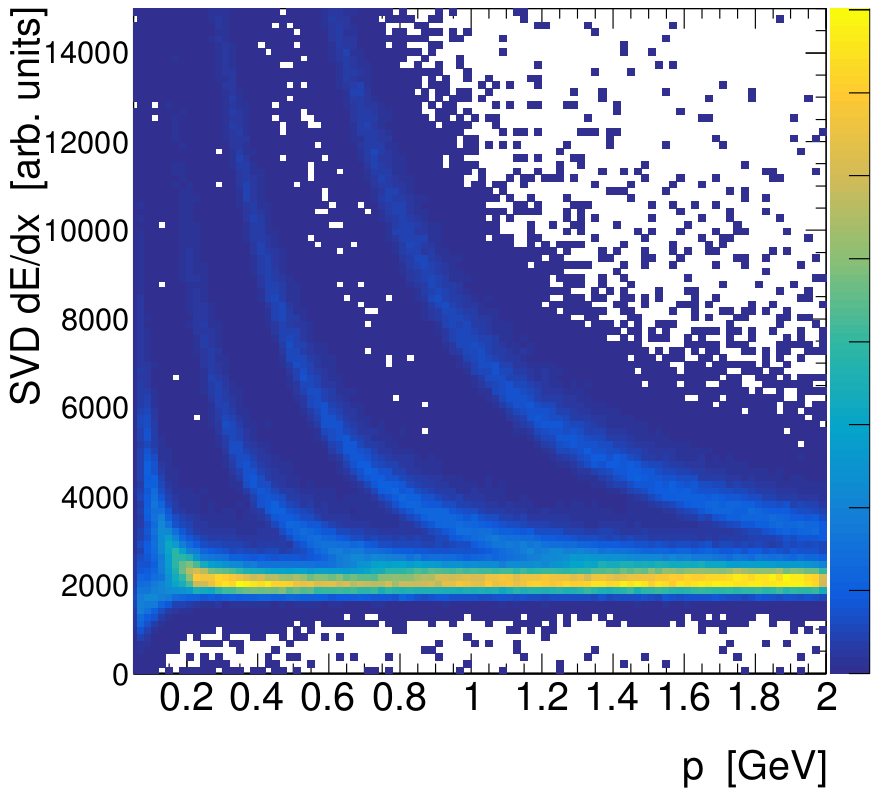
\includegraphics[width=0.43\textwidth,height=\textheight,keepaspectratio]{{{../res/dE dx for SVD detector by particles}}}
	}
	\hspace{2em}
	\subcaptionbox{$E/p$\label{fig:e_p_for_ECL}}{
		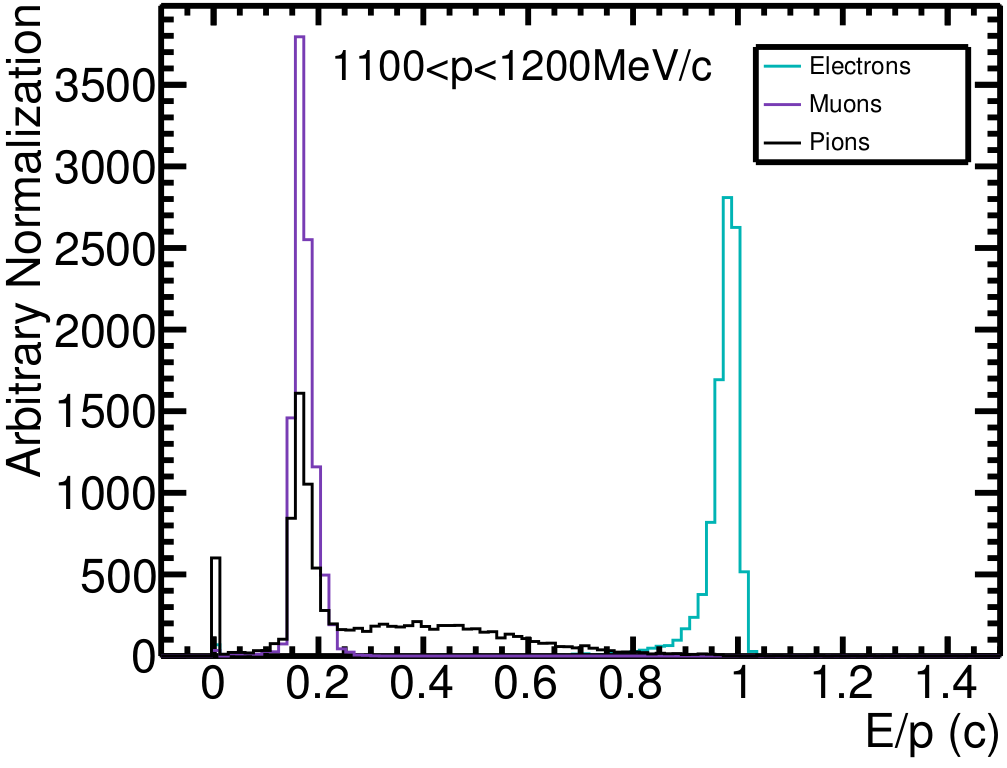
\includegraphics[width=0.43\textwidth,height=\textheight,keepaspectratio]{{{../res/E p for ECL detector by particles}}}
	}
	\caption[Separation of different particle species for various simulated signals. Taken from~\cite{Belle2Collaboration:B2TiP}.]{
		Separation of different particle species for various simulated signals. Taken from~\cite{Belle2Collaboration:B2TiP}.

		\textbf{Figure~\subref{fig:de_dx_for_SVD}} shows the $\mathrm{d}E/\mathrm{d}x$ means as a function of momentum in the SVD with the color encoding the number of hits. In order to reduce outliers the lowest $5\%$ and highest $25\%$ of the measurements of each track are not used in the estimation.

		\textbf{Figure~\subref{fig:e_p_for_ECL}} shows the $E/p$ distribution for different particle species.
	}
\end{figure}

\chapter{Statistics for particle analysis}
\label{chap:statistics}

\section{Classification functions}
\label{sec:classification_functions}

A main part of identifying particles is to examine statistical measures. The main concepts used throughout the thesis heavily relies on such values to compare the goodness of a identification method. However their use is not limited to physics, let alone particle physics, but spans over all field containing some form of (binary) classification problems.
In the following explanatory paragraphs it is assumed that one wants to identify kaons in a set of data containing a multitude of alternative particles.

The most important classification functions are:
\begin{itemize}
	\item \textbf{T}rue \textbf{P}ositive \textbf{R}ate (\textbf{TPR}): \textit{Proportion of accepted elements which are correct relative to all positives}

	\nobreak
	Hence the ratio of identified kaons which actually were kaons in proportion to the number of kaons in the data.

	\item \textbf{T}rue \textbf{N}egative \textbf{R}ate or Specificity (\textbf{TNR}): \textit{Proportion of rejected elements which are incorrect relative to all negatives}

	\nobreak
	In our example this would translate to the ratio of non-kaon particles being identified as non-kaons in proportion to the number of all non-kaon particles.

	\item \textbf{F}alse \textbf{P}ositive \textbf{R}ate (\textbf{FPR}): \textit{Proportion of accepted elements which are incorrect relative to all negatives}

	\nobreak
	This would translate to the fraction of non-kaon particles identified as kaons over the number of all non-kaons.

	\item \textbf{F}alse \textbf{N}egative \textbf{R}ate (\textbf{FNR}): \textit{Proportion of rejected elements which are correct relative to all positives}

	\nobreak
	Using our kaon sample once more; this would represent the fraction of kaons classified as being non-kaons over the number of all non-kaons.

	\item \textbf{P}ositive \textbf{P}redicted \textbf{V}alue (\textbf{PPV}): \textit{Proportion of accepted elements which are correct relative to all accepted}

	\nobreak
	Using our kaon sample one last time; this would represent the fraction of kaons classified as being as kaons over the number of all tracks classified as kaons but not necessarily being one.

\end{itemize}

In abstract terms; the two prefixes used above may be summarized as seen in \autoref{tab:classification_guidelines}. Bear in mind that `negative' and `positive' if used separately denote the presence of the desired feature and therefore does not fit the definition given in the table in this case.

\begin{table}[ht]
	\centering
	\begin{tabular}{l|ll}
		Veracity & True = correct & False = incorrect \\
		Identification & Positive = accepted & Negative = rejected
	\end{tabular}
	\caption{Guidelines for understanding the meaning of a classification function.}
	\label{tab:classification_guidelines}
\end{table}

\section{Receiver operating characteristic}
\label{sec:roc}

The \textbf{R}eceiver \textbf{O}perating \textbf{C}haracteristic (\textbf{ROC}) curve is the TPR plotted over the FPR. As such the values on the $x$ and $y$ axis go from $0$ to $1$. Each point on the curve represent an applied selection criterion on the data.

On a set of data with two equally likely yields a straight diagonal line connecting the point $(0, 0)$ with $(1, 1)$ would represent plain guessing. A curve below that would be worse and anything above, is some degree of good. An optimal curve would achieve a high TPR value at a very low FPR.
Multiple methods can therefore be compared by assessing how steep each methods TPR is rising relative to the FPR. The \autoref{fig:sample_roc_curve} visually underlines the above described relations.

\begin{figure}[ht]
	\centering
	\includegraphics[width=\textwidth,height=0.4\textheight,keepaspectratio]{{{../res/Sample Receiver Operating Characteristic (ROC) curve}}}
	\caption{Sample ROC curve for a binary classification problem with each outcome being equally likely.}
	\label{fig:sample_roc_curve}
\end{figure}

\section{Identification efficiencies}
\label{sec:efficiency}

In particle physics the identification efficiency is defined as the proportion of correctly classified particles relative to all the available particles belonging to that class. Hence it directly represents the PPV. Both terms will be used as synonyms throughout the thesis.

For an exclusive particle classification the $\epsilon_{PID}$-matrix is the confusion matrix normed by row. Each cell in a row represents the probability of a particle of that row's class being identified as the particle of that column's class. On the diagonal of that matrix it contains the identification efficiencies for a particle species.
The definition generalizes to non normed matrices, e.g. resulting from non-exclusive. Although reading the matrix is less intuitive as a particle might belong to multiple classes and makes comparing them very ambitious.

The values of the matrix are given by the fraction of particles $i$ classified as $j$ over the true abundance of particle $i$. As formula its values are

\begin{equation}
	\epsilon_{i j} = \frac{N_{i \text{ classified as } j}}{A_{i \text{ true}}}.
\end{equation}

For our six particle species with ID the matrix has the following shape:

\begin{equation}
	\begin{pmatrix}
		\epsilon_{K K} & \epsilon_{K \pi} & \epsilon_{K e} & \epsilon_{K \mu} & \epsilon_{K p} & \epsilon_{K d} \\
		\epsilon_{\pi K} & \epsilon_{\pi \pi} & \epsilon_{\pi e} & \epsilon_{\pi \mu} & \epsilon_{\pi p} & \epsilon_{\pi d} \\
		\epsilon_{e K} & \epsilon_{e \pi} & \epsilon_{e e} & \epsilon_{e \mu} & \epsilon_{e p} & \epsilon_{e d} \\
		\epsilon_{\mu K} & \epsilon_{\mu \pi} & \epsilon_{K e} & \epsilon_{K \mu} & \epsilon_{K p} & \epsilon_{\mu d} \\
		\epsilon_{p K} & \epsilon_{p \pi} & \epsilon_{p e} & \epsilon_{p \mu} & \epsilon_{p p} & \epsilon_{p d} \\
		\epsilon_{d K} & \epsilon_{d \pi} & \epsilon_{K e} & \epsilon_{K \mu} & \epsilon_{K p} & \epsilon_{d d} \\
	\end{pmatrix}.
\end{equation}

\section{Likelihood}
\label{sec:likelihood}

\subsection{Likelihood ratio}
\label{subsec:likelihood_ratios}

The ratio of likelihoods is commonly used for comparisons of the goodness of two models. Consider two alternative models, one parameterised by the hypothesis $H_0$, the other by $H_1$. Each yield a likelihood of event $\pmb{x}$ occurring given their hypothesis is true. Their ratio
\begin{equation*}
	\frac{\mathcal{L}(\pmb{x}|H_0)}{\mathcal{L}(\pmb{x}|H_1)}
\end{equation*} denotes how many times more likely the event $\pmb{x}$ is under hypothesis $H_0$ relative to $H_1$.

However the event $\pmb{x}$ must not necessarily take the form a simple one dimensional value. It may very well be a composition of e.g. in our case multiple detectors responses. Nevertheless if one assumes all constituents $x_i$ of $\pmb{x}$ are independent of each other, one may simple construct $\mathcal{L}(\pmb{x}|H_0)$ by multiplying the separate likelihoods of each $x_i$ given that $H_0$ is true:
\begin{equation*}
	\mathcal{L}(\pmb{x}|H_0) = \prod \limits_{i} \ell_i(x_i|H_0).
\end{equation*}
In out case $\mathcal{L}(\pmb{x}|H_0)$ might be seen as the likelihood of measuring a signal given a particle hypothesis is true. It value would be constructed by multiplying the likelihoods of $\ell(x_i|H_0)$ for each detector $i$.

\subsection{Neyman-Pearson}
\label{subsec:likelihood_ratios_neyman_pearson}

When separating two models which have no unknown parameters the Neyman-Pearson lemma states that a test on the likelihood ratio has the highest probability of correctly rejecting the original hypothesis if the alternative hypothesis is indeed true. In other words it states that a test on the likelihood ratio providing the highest purity at a given efficiency.

\section{Neural network}
\label{sec:neural_network}

A neural network or more precisely an artificial neural network is an algorithm inspired by the central nerve system of biological beings. However instead of electrical signals being passed on from neuron to neuron with complex biological process involved in summing up incoming systems, an artificial neural network passes on numbers with functions representing neurons.

Despite this simplistic design a neural network can get complicated fast. The most simplest approach would be to just stacking multiple layers of neurons (\textit{nodes}) on top of each other and connecting the outputs of the previous layer with those new nodes (feed-forward neural network). However a network can in theory be designed arbitrarily deep and provide a multitude of additional feedback loops (recurrent neural network) and further binning restrictions of node-inputs (convolutional neural network).

\begin{figure}[ht]
	\centering
	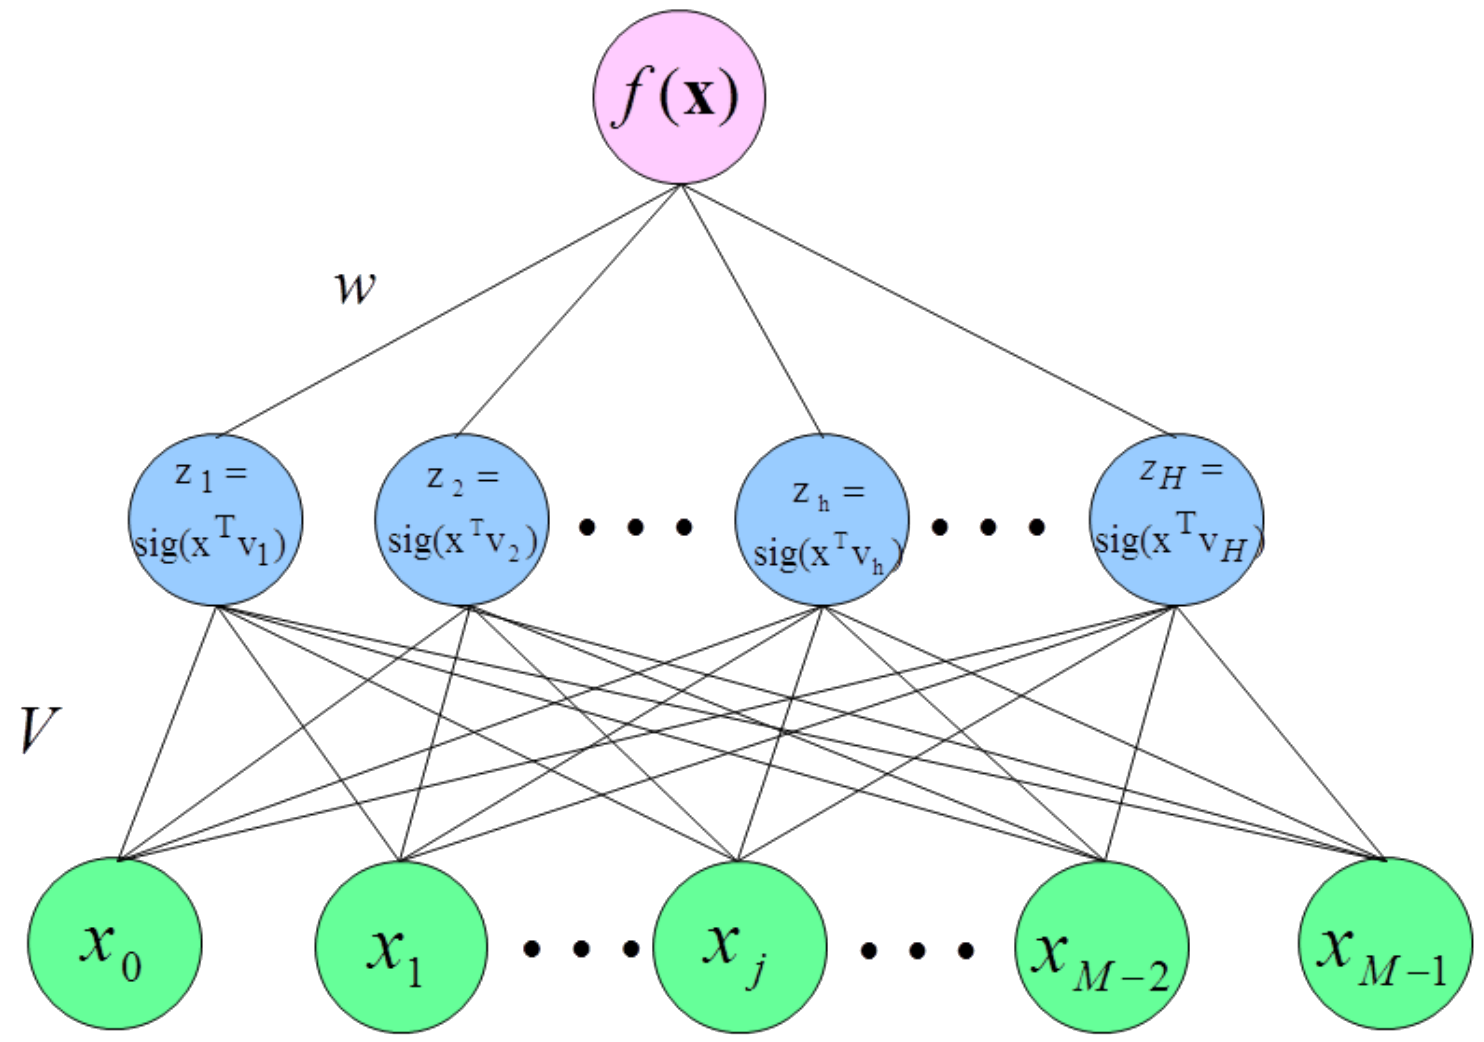
\includegraphics[width=\textwidth,height=0.4\textheight,keepaspectratio]{{{../res/Design of an artificial neural network}}}
	\caption{Design of an artificial neural network with one layer, $\pmb{x}$ as input, $z_i$ as activation function, $V$ und $w$ as weights and $f(\pmb{x})$ as prediction. Taken from~\cite{MachineLearning:NeuralNetworks}.}
	\label{fig:sample_neural_network_design}
\end{figure}

A rather simple feed-forward network is depicted in \autoref{fig:sample_neural_network_design}. Each line between two bubbles represents a connection, meaning the output of the bubble at the bottom is passed to the bubble at the top. The function used in calculating the various values for $z_i$ is called sigmoid (see~\cite{MachineLearning:NeuralNetworks}) and has an S-like shape. In terms of biology it can be though of as a boundary which has to be overcome prior to a signal being passed on. The references in the following paragraph are in regards to this figure.

Layers not representing the input or output are called hidden layers ({\color{blue}blue bubbles}). However the dimensions of an input ({\color{green}green bubbles}) are also referred to as features. The function of a node is called \textit{activation function} ($z_i$). The term \textit{learning} in the context of neural network refers to the process of adapting parameters or \textit{weights} ($V$ and $w$) of a nodes via a gradient which optimizes the desired function. The desired function is usually referred to as \textit{loss} and e.g. describes how many false classifications have been made. It is the job of the \textit{optimizer} to adapt the weights in a way which minimizes the function, a task usually done via propagating the error back through the network in a schema called \textit{back propagation}. The term \textit{training} refers to the process of applying the network to a set of data and adjusting the weights as necessary for each iteration. How many individual data points one of those iterations contains is described by the \textit{batch size}.

\chapter{Analysis}
\label{chap:analysis}

\section{Data sample}
\label{sec:data_sample}

In order to validate a particle identification approach and to make sure it is behaving as expected, it is good practice to measure the performance on Monte Carlo simulated data. The software framework EvtGen is used for the purpose of simulating the production and the decay of the $\Upsilon(4S)$. The subsequent generic decay is simulated using decay files provided by the Belle~\RN{2} software. After the simulation of the particle and their various properties, the detector responses are emulated. Hits in the various detector components are simulated and finally the veracity of a track identification is calculated. The process of matching the identification with the truth is not possible for real data, as the true property of a particle are not known in the experiment. However, for testing purposes it is a valuable tool as it allows to compare the performance of new approachs.

Throughout the thesis several decays are discussed, most notably the decay of the charged $B$ mesons. $\Upsilon(4S)$ decays in $(51.4 \pm 0.6) \%$ of cases into the charged $B^+$ and $B^-$. Therefore it represents a good sample of the overall to be expected particle species. Observations seen in this generic charged decay were validated using data of the `mixed' decay of the $B$ meson into $B^0$ and $\bar{B}^0$ which has a branching ratio of $(48.6 \pm 0.6) \%$. Both samples are generic decays and not specific to one analysis. A complete list of possible decay-strings as well as the above mentioned branching fractions can be found in~\cite{Patrignani:2016xqp}.

Additionally a simulated decay of the $B^+ B^-$ with non-generic properties is generated. Its properties are outlined in \autoref{tab:simulated_decay}. It allows for a fast processing of tests due to its simplicity and helps in differentiating between decay specific observations and generic ones. The data from this decay is not used for visualizations as it does not translate to an application in the real world.

\begin{table}[ht]
	\centering
	\begin{tabular}{l|l}
		Decay string & Branching ratio \\
		\hline
		$\Upsilon(4S) \rightarrow B^+ B^-$ & $1.$ \\
		\quad $B^+ \rightarrow \mu^+ \nu_{\mu} \gamma$ & $1.$ \\
		\quad $B^- \rightarrow \pi^- D^0$ & $1.$ \\
		\qquad $D^0 \rightarrow K^- \pi^+$ & $0.2$ \\
		\qquad 	$D^0 \rightarrow K^- \pi^+ \pi^0$ & $0.2$ \\
		\qquad 	$D^0 \rightarrow K^- \pi^+ \pi^+ \pi^-$ & $0.2$ \\
		\qquad 	$D^0 \rightarrow K^- K^+$ & $0.2$ \\
		\qquad 	$D^0 \rightarrow \pi^+ \pi^0$ & $0.2$ \\
	\end{tabular}
	\caption{Simulated non-generic decay of the $\Upsilon(4S)$ with charge conjugated decays implied.}
	\label{tab:simulated_decay}
\end{table}

As seen in \autoref{fig:true_particle_abundance} the decays are dominated by kaons and pions. However, the overall distribution is much more peaked for the charged generic decay. Furthermore the non-generic sample decay features a feature a lot more $\mu^+$ relatively speaking in comparison charged generic decay. The mixed generic decay is disregarded for this plot due to its distinct similarity to the charged decay.

\begin{figure}[ht]
	\centering
	\subcaptionbox{Charged\label{fig:charged_decay_true_particle_abundance}}{
		\includegraphics[width=0.43\textwidth,height=\textheight,keepaspectratio]{{{../res/charged 01/General Purpose Statistics: True Particle Abundances in the K+-Data}}}
	}
	\hspace{2em}
	\subcaptionbox{Sample\label{fig:sample_decay_true_particle_abundance}}{
		\includegraphics[width=0.43\textwidth,height=\textheight,keepaspectratio]{{{../res/sample/General Purpose Statistics: True Particle Abundances in the K+-Data}}}
	}
	\caption{True particle abundance in various simulated decays with particle on the $x$-axis sorted by their frequency. \textit{NaN} stands for an invalid translation\protect\footnotemark from the particles' PDG code to an actual particle.}
	\label{fig:true_particle_abundance}
\end{figure}
\footnotetext{The error occurs due to the PDG code in the ROOT file being saved as \lstinline|float32|. However, some particle's code exceed the memory limit of $32$-bits. Notably this effects the deuteron and its anti-particle.}

Prior to evaluating the data, it is stripped of falsely identified and poorly defined tracks. First the transverse momentum is limited to the range of $0.0$ to $5.29$. This removes very slow and very fast particles as both provide very badly described tracks. Next, the transverse distance of the closest point of the track to the point of interaction is limited to $2 \mathrm{~cm}$, respectively $5 \mathrm{~cm}$ for the longitudinal distance. Lastly, tracks with no assigned PDG code are pruned. Such tracks are considered falsely reconstructed as a majority of hits of the track do not belong to the true simulated track. Including those kinds of tracks would have suggested the particle identification process shall identify non-particles tracks. Overall the effect of tracks with no PDG code does not influence the final result in any significant way. The tracks were merely excluded for the purpose of clarity.

The generic decay files are used in the following discussion. Each decay file features $100,000$ initial $B \bar{B}$ events and about ten times as many identified tracks. The non-generic decay contains $10,000$ initial events and about $40,000$ tracks.

If not specifically otherwise stated it can be assumed that the graphs and visuals in the following paragraphs are based on the data from one generic charged decay file. The number of samples in one such file is sufficiently high for the purpose of the study while still providing acceptable performance.

\section{Particle identification variables}
\label{sec:pid_variables}

\subsection{Legacy PID}
\label{subsec:pid_variables_legacy_pid}

The current particle identification approach consists of variables calculated via ratios of likelihoods. A particle identification is performed by applying a selection, also called \textit{cut} on the variables.

As of \formatdate{28}{06}{2018}, the current approach is to take the likelihood of the desired particle and divide it by itself plus the likelihood of the pion. To construct the ID of the pion the kaon likelihood is used as second summand in the denominator. \autoref{tab:legacy_particleid_variables} shows the definition of the ID for each of the six particle species of interest. In the future it will be replaced by the global PID approach, described in \autoref{subsec:pid_variables_global_pid}.

\begin{table}[ht]
	\centering
	\begin{tabular}{l|l}
		pionID & $\mathcal{L}_{\pi} / (\mathcal{L}_{\pi} + \mathcal{L}_{K})$ \\
		kaonID & $\mathcal{L}_{K} / (\mathcal{L}_{K} +\mathcal{L}_{\pi})$ \\
		protonID & $\mathcal{L}_{p} / (\mathcal{L}_{p} +\mathcal{L}_{\pi})$ \\
		electronID & $\mathcal{L}_{e} / (\mathcal{L}_{e} +\mathcal{L}_{\pi})$ \\
		muonID & $\mathcal{L}_{\mu} / (\mathcal{L}_{\mu} +\mathcal{L}_{\pi})$ \\
		deuteronID & $\mathcal{L}_{d} / (\mathcal{L}_{d} +\mathcal{L}_{\pi})$
	\end{tabular}
	\caption{Definition of the ParticleID variables currently used by default for particle identification.}
	\label{tab:legacy_particleid_variables}
\end{table}

The identification efficiencies for pions and kaons are rather good as the approach is able to properly differentiate both classes. However, it has obvious limitations in identifying rare particles as the fraction is dominated by the high abundance of the pion.

The difference in the TPR for identifying the pions and the electron can be seen in \autoref{fig:legacy_pid_particle_identification}. The pions is used as a representative of a particle specie with a high abundance, while the electron is one of the low abundance particle species. A high efficiency in selecting the particles is achieved quickly. However, the purity of the sample clearly underlines the preference towards the pion identification.

\begin{figure}[ht]
	\centering
	\subcaptionbox{Pion identification\label{fig:legacy_pid_pions_identification}}{
		\includegraphics[width=0.4\textwidth,height=\textheight,keepaspectratio]{{{../res/charged 01/Particle ID Approach: pi Identification}}}
	}
	\hspace{2em}
	\subcaptionbox{Electron identification\label{fig:legacy_pid_electron_identification}}{
		\includegraphics[width=0.4\textwidth,height=\textheight,keepaspectratio]{{{../res/charged 01/Particle ID Approach: e Identification}}}
	}
	\caption{Particle identification rates for the pions and electron using the legacy PID approach, each showing the True Positive Rate (ROC curve) and the Positive Predicted Value depending on the False Positive Rate.}
	\label{fig:legacy_pid_particle_identification}
\end{figure}

This unbalanced classification is further emphasized by analyzing the identification efficiencies. The matrix shown in~\autoref{fig:legacy_pid_epsilon_pid} clearly highlights the bias of the classification towards kaons and pions. There is a high chance of a particle being identified as kaon or pion, regardless of the actual particle's identity.

\begin{figure}[ht]
	\centering
	\includegraphics[width=\textwidth,height=0.3\textheight,keepaspectratio]{{{../res/charged 01/Particle ID Approach: Heatmap of epsilonPID Matrix for an exclusive Cut}}}
	\caption{Matrix of $\epsilon$ values for the legacy particle ID approach.}
	\label{fig:legacy_pid_epsilon_pid}
\end{figure}

\subsection{global PID}
\label{subsec:pid_variables_global_pid}

The global PID approach is the upcoming approach which is to be used as new default variable on which to select particle samples. Instead of having the likelihood of the pion fixed in the denominator of every particle's id, it is replaced by the sum over all the other particles. Hence, the global PID of the kaon is now represented by the likelihood of the kaon divided by sum of all the likelihoods of every other particle including the kaon itself. The complete list of the definition can be seen in \autoref{tab:global_pid_variables}.

\begin{table}[ht]
	\centering
	\begin{tabular}{l|l}
		globalPionID & $\mathcal{L}_{\pi} / \mathcal{L}_{all}$ \\
		globalKaonID & $\mathcal{L}_{K} / \mathcal{L}_{all}$ \\
		globalProtonID & $\mathcal{L}_{p} / \mathcal{L}_{all}$ \\
		globalElectronID & $\mathcal{L}_{e} / \mathcal{L}_{all}$ \\
		globalMuonID & $\mathcal{L}_{\mu} / \mathcal{L}_{all}$ \\
		globalDeuteronID & $\mathcal{L}_{d} / \mathcal{L}_{all}$ \\
		\hline
		\multicolumn{2}{c}{$\mathcal{L}_{all} = \sum \limits_{x \in {\pi, K, p, e, \mu, d}} \mathcal{L}_{x}$}
	\end{tabular}
	\caption{Definition of the globalPID variables which is to be used by default for particle identification in the future.}
	\label{tab:global_pid_variables}
\end{table}

The approach is not biased towards merely differentiating between kaons and pions but instead has a more balanced classification. Every likelihood of a particle specie has the same weight in the denominator.

\subsection{Goodness of the global PID variables}
\label{subsec:pid_variables_global_pid_goodness}

In order to ensure the global PID variables are properly defined, a likelihood ratio test based on the Neyman-Pearson lemma as outlined in \autoref{subsec:likelihood_ratios_neyman_pearson} is used. The lemma states that the highest purity for a given efficiency is to be expected for each selection on the likelihood ratio as seen in \autoref{fig:neyman_pearson_visualization}.

For the following analysis the data is sampled into $10$ bins of equal height as to provide a balanced statistics for each bin. The error in a bin is given by a vertical line. It is calculated via gaussian error propagation under the assumption that the counting of the events follow a Poisson distribution. Thereby assumption is made that the number of desired particles in a bin and the number of undesired particles are independent. The error is underestimated for a purity of $0$ and $1$.

When applying the previously discussed approach to the data, the goodness of the likelihoods can be validated as seen in \autoref{fig:likelihood_ratio_kaon_all}. The purity of the kaon sample in the bins increases with a stricter likelihood cut and the uncertainty is low due to the high statistics. However, \autoref{fig:likelihood_ratio_proton_all} paints a completely different picture. The purity peaks at a likelihood ratio of about $0.35$, while the following values are far lower. However, this effect is unique to the proton and can not be observed in any other of the six particle species of interest. On one the hand this means the likelihoods for the kaon, pion, electron, muon and deuteron are properly defined and actually behave like probabilities. On the other hand it also reveals a flaw in the calculation of the proton likelihood. Thankfully the proton does not play a significant role in the analysis done in the following sections but nevertheless it is important to keep in mind that identifying protons via their likelihood (likelihood ratio) has inherent flaws.

\begin{figure}[ht]
	\centering
	\subcaptionbox{Kaon\label{fig:likelihood_ratio_kaon_all}}{
		\includegraphics[width=0.4\textwidth,height=\textheight,keepaspectratio]{{{../res/charged 01/pidProbability Approach: Relative K Abundance in Likelihood Ratio Bins for ALL detector}}}
	}
	\hspace{2em}
	\subcaptionbox{Proton\label{fig:likelihood_ratio_proton_all}}{
		\includegraphics[width=0.4\textwidth,height=\textheight,keepaspectratio]{{{../res/charged 01/pidProbability Approach: Relative p Abundance in Likelihood Ratio Bins for ALL detector}}}
	}
	\caption{Relative abundance (purity) of various particle samples in likelihood ratio bins.}
	\label{fig:likelihood_ratio_all}
\end{figure}

In order to understand the observed effect in \autoref{fig:likelihood_ratio_proton_all} it is important to pin down its cause. Since the likelihoods are values which are returned by each detector, a natural conclusion might be that it is caused by one poorly defined detector response. \autoref{fig:likelihood_ratio_proton_by_detector} shows the relative abundance of the proton in likelihood ratio bins for various detector components.

\begin{figure}[ht]
	\centering
	\subcaptionbox{SVD\label{fig:likelihood_ratio_proton_svd}}{
		\includegraphics[width=0.4\textwidth,height=\textheight,keepaspectratio]{{{../res/charged 01/pidProbability Approach: Relative K Abundance in Likelihood Ratio Bins for SVD detector}}}
	}
	\hspace{2em}
	\subcaptionbox{CDC\label{fig:likelihood_ratio_proton_cdc}}{
		\includegraphics[width=0.4\textwidth,height=\textheight,keepaspectratio]{{{../res/charged 01/pidProbability Approach: Relative p Abundance in Likelihood Ratio Bins for CDC detector}}}
	}

	\subcaptionbox{TOP\label{fig:likelihood_ratio_proton_top}}{
		\includegraphics[width=0.4\textwidth,height=\textheight,keepaspectratio]{{{../res/charged 01/pidProbability Approach: Relative p Abundance in Likelihood Ratio Bins for TOP detector}}}
	}
	\hspace{2em}
	\subcaptionbox{ARICH\label{fig:likelihood_ratio_proton_arich}}{
		\includegraphics[width=0.4\textwidth,height=\textheight,keepaspectratio]{{{../res/charged 01/pidProbability Approach: Relative p Abundance in Likelihood Ratio Bins for ARICH detector}}}
	}

	\subcaptionbox{ECL\label{fig:likelihood_ratio_proton_ecl}}{
		\includegraphics[width=0.4\textwidth,height=\textheight,keepaspectratio]{{{../res/charged 01/pidProbability Approach: Relative p Abundance in Likelihood Ratio Bins for ECL detector}}}
	}
	\hspace{2em}
	\subcaptionbox{KLM\label{fig:likelihood_ratio_proton_klm}}{
		\includegraphics[width=0.4\textwidth,height=\textheight,keepaspectratio]{{{../res/charged 01/pidProbability Approach: Relative p Abundance in Likelihood Ratio Bins for KLM detector}}}
	}

	\caption{Relative abundance (purity) of the proton in likelihood ratio bins for all available detectors.}
	\label{fig:likelihood_ratio_proton_by_detector}
\end{figure}

The response of the SVD is in perfect agreement with the expectation. However, the CDC shows the same kink merely shifted a little to the left. The TOP is in agreement again. The ARICH, ECL and KLM have an insufficient statistics and/or the likelihoods do not fil the whole range. The error is underestimate at multiple points close to a purity of $0$. Hence the ECL seems like the only viable cause of the unexpected kink in the proton purity over likelihood ratio plot. The observed shift to the left is due to the likelihood of a single detector in general being lower than the  likelihood of all detectors combined.

Next, the $p_t$ dependency in the CDC detector was analysed as depicted in \autoref{fig:likelihood_ratio_proton_by_pt}. As sampling method three equal height bins are chosen. Using rather few bins with the same number of particles in each one, provides good statistics and allows for fair comparisons. Analyzing the picture, it becomes obvious that especially low to medium transverse momentum protons constitute to the effect.

\begin{figure}[ht]
	\centering
	\includegraphics[width=\textwidth,height=0.5\textheight,keepaspectratio]{{{../res/charged 01/pidProbability Approach: Relative p Abundance in Likelihood Ratio Bins for CDC detector for equal size pt bins}}}
	\caption{Relative abundance of the proton in likelihood ratio bins for different transverse momentum ranges in units of $GeV/c$ for the CDC detector.}
	\label{fig:likelihood_ratio_proton_by_pt}
\end{figure}

Furthermore it is important to bear the locations of the detector components in mind. Of special interest in this case is the end of the TOP detector, at roughly $(- 60^{\circ})$ relative to the beampipe (see~\autoref{fig:belle2_detector_design_white_paper}). At this point the particle identification gets notably different. However, as this effects all tracks equally for $p_t$ bins it cancels out in comparisons. The effect becomes important for equal height bins of the angle.

In conclusion the likelihood of the proton returned by the CDC detector should be seen with healthy skepticism and not be taken for granted as it does not behave as a likelihood. Further analysis needs to take place in order to pin down the actual cause.

\section{Bayesian approach}
\label{sec:bayesian_approach}

\subsection{Simple Bayes}
\label{subsec:bayesian_approach_simple_bayes}

The idea for this approach is inspired by the work done at the ALICE experiment as outlined in~\cite{Adam:2016acv} and~\cite{Belikov:2005zz}.

The goal of a Bayesian approach is to weight the particles' probability by their abundance in the sample. This process increases the likelihood of a particle being identified as belonging to a group with a higher abundance and decreases the likelihood of being identified as belonging to a group with a lower abundance. Bayes theorem provides the mathematical foundation:
\begin{equation*}
	\displaystyle P(A|B) = \frac{P(B|A) \cdot P(A)}{P(B)}
	\text{,}
	\qquad
	\text{e.g.,} \quad P(e|Signal) = \frac{P(Signal|e) \cdot P(e)}{P(Signal)}.
\end{equation*}
The variable $P(e|Signal)$ is the probability of the track being from an electron given that $Signal$ is measured. The part of most interest in the equation is the a priori probability $P(A)$, respectively $P(e)$. As a first simple approach this variable is now dependant on the absolute abundance of electrons. The probability of detecting the signal is modeled using
\begin{equation*}
	P(Signal) = \sum \limits_{x \in {\pi, K, p, e, \mu, d}} P(Signal|x) \cdot P(x)
\end{equation*}
with $P(Signal|x)$ being the previously discussed likelihoods of the signal using the particle hypothesis $x$. Note that the absolute normalization of $P(x)$ cancels out as it occurs in both nominator and denominator. Therefore, it makes no difference if the value of the abundance is used directly as $P(x)$ in the calculation.

The absolute particle abundance of a sample taken from the Monte Carlo simulation of the charged decay of the $B$-mesons can be seen in \autoref{fig:charged_decay_true_particle_abundance}. In this example the bias towards pions and kaons can be clearly observed.

The approach depends on the detector yielding decay-agnostic results. Hence the detector shall be assumed to always output the likelihood of measuring the received signal given a specific particle hypothesis regardless of prior probabilities. Furthermore the approach assumes a bias towards one or a few particles in the data since otherwise the a priori probabilities would be flat and would have no effect.
Thankfully both of those hypothesis are fulfilled in the real world: The detector can be assumed to behave independently of the relative particle abundance and the measured data shows a clear predominance of one or a few particle species. This is not surprising in itself as the branching fractions are not equally distributed.

\subsection{Univariate Bayes}
\label{subsec:bayesian_approach_univariate_bayes}

The univariate Bayesian approach adds a further dependency in the form of a detector variable to the a priori probabilities of the Bayesian approach. Hence, instead of having a priori probability which depends only on the particle overall abundance, the univariate approach additionally varies the value. Namely the abundance is made dependant on, e.g., the transverse momentum and the angle between the beampipe and track $\Theta$ are considered. Those two variables make the most sense as they play a significant role in the track fitting process and are dominant factors for the particle classification process outlined in~\autoref{subsec:particle_identification}. In the following, the cosine of $\Theta$ is used in order to even out the distribution.

\begin{figure}[ht]
	\centering
	\subcaptionbox{$p_t$\label{fig:univariate_bayes_priors_by_pt}}{
		\includegraphics[width=0.4\textwidth,height=\textheight,keepaspectratio]{{{../res/charged 01/Univariate Bayesian Approach: K Spectra Ratios Relative to pi for pt bins}}}
	}
	\hspace{2em}
	\subcaptionbox{$\cos(\Theta)$\label{fig:univariate_bayes_priors_by_costheta}}{
		\includegraphics[width=0.4\textwidth,height=\textheight,keepaspectratio]{{{../res/charged 01/Univariate Bayesian Approach: K Spectra Ratios Relative to pi for cos(Theta) bins}}}
	}
	\caption{Kaon abundance relative to the pion abundance in equal height bins of $p_t$ and $\cos(\Theta)$ with horizontal lines indicating the size of each bin.}
	\label{fig:univariate_bayes_priors}
\end{figure}

The relative abundance of one particle in comparison to the pion is shown in \autoref{fig:univariate_bayes_priors}. Equal height bins were chosen to enforce a good statistics across all bins. The abundance relative to the pion is used in order to introduce a point of reference. The pion as such reference point is chosen arbitrarily. As previously discussed, the absolute normalization of the a priori probabilities does not matter. The graphs underline the motivation for using such an approach as the abundance varies between different bins. Especially the dependency on $p_t$ reveals drastic changes in the relative frequency of the kaon. Overall binning by $p_t$ reveals shows a higher contrast and therefore is used as default binning method.

Due to its additional dependency the univariate Bayesian approach is able to adapt to the underlying data a little better in comparison to the Bayesian approach.

\subsection{Multivariate Bayes}
\label{subsec:bayesian_approach_multivariate_bayes}

The multivariate approach extends the univariate one by further increasing the number of free parameters on which the a priori probabilities may depend on. As previously mentioned both $p_t$ and $\cos(\Theta)$ make for an excellent choice as default variables for said dependency. Those variables provide a good separation between different particle species for certain pockets.

\begin{figure}[ht]
	\centering
	\includegraphics[width=\textwidth,height=0.4\textheight,keepaspectratio]{{{../res/charged 01/Multivariate Bayesian Approach: Multi-axes Histogram of pt, cosTheta for e, K, pi}}}
	\caption{Scatter plot with tracks represented as opaque points depending on $p_t$ and $\cos(\Theta)$. The color encodes the specie of the particle.}
	\label{fig:multivariate_bayes_multi_axis_histogram_by_pt_by_costheta}
\end{figure}

\autoref{fig:multivariate_bayes_multi_axis_histogram_by_pt_by_costheta}~shows tracks as transparent dots scattered across the plane, accompanied by two histograms showing the distribution in transverse momentum and the cosine of the angle between beampipe and track. It is important to note the sickle shape of the distribution. Higher values of the cosine are slightly preferred over lower ones due to the asymmetry of the beams. Furthermore the visual highlights the fact that angles of about $90^{\circ}$ ($\cos(\Theta) = 0$) correspond to the highest transverse momentums. In addition a slight separation between the yellow sickle on the left (pions), the cyan  in the middle (kaons) and the violet sickle on the right (electrons). The tail of the pion sickle extens beyond both kaons and electrons but it far less frequent. Intuitively this makes sense since as the production of a heavier particle\footnotemark consumes a more phase space which in turn reduces the amount of momentum it can carry. Analog, the electron is relatively speaking lightweight and therefore may carry a lot of momentum (not necessarily transverse momentum though). Obviously this interpretation disregards the fact that particles are not created one by one, but rather in a complex decay and the phase space is distributed across all daughters. Nevertheless, it illustrates the observed effect.
\footnotetext{Note, the mass of the kaon is about three and a half times higher than the mass of the pion.}

Enabling the a priori probability to depend on those measurements allows it to pick more fine grained priors. The a priori probabilities are estimated according using the Monte Carlo information for each combination of variables. In order to achieve this the variable $p_t$ and $\cos(\Theta)$ were distributed across equal height bins and the relative abundance of each particle relative to the pion were calculated for every combination of $p_t$ and $\cos(\Theta)$ bin.

\begin{figure}[ht]
	\centering
	\includegraphics[width=\textwidth,height=0.4\textheight,keepaspectratio]{{{../res/charged 01/Multivariate Bayesian Approach: K Spectra Ratios Relative to pi}}}
	\caption{Relative kaon abundance in equal height transverse momentum and cosine of $\Theta$ bins.}
	\label{fig:multivariate_bayes_k_spectra_relative_to_pi}
\end{figure}

The abundance of kaons relative to the abundance of pions can be seen in~\autoref{fig:multivariate_bayes_k_spectra_relative_to_pi}. The graph emphasizes the fact that particles abundances are unevenly distributed across the $p_t$-, $\cos(\Theta)$-plane. The additional information contained in the newly added variables may be used for an improved classification of the tracks.

\subsection{Comparison}
\label{subsec:bayesian_approach_comparison}

\begin{figure}[ht]
	\centering
	\includegraphics[width=\textwidth,height=0.4\textheight,keepaspectratio]{{{../res/charged 01/Diff Statistics: pi Identification via legacy PID, via simple Bayes}}}
	\caption{Comparison of PPV, TPR and FPR for simple Bayes with legacy PID approach for identifying pions. The upper graph shows both rates of each approach separately using different colors, while the lower visualizes the ratio between the PPV's respectively the TPR's.}
	\label{fig:diff_stats_pi_identification_via_pid_via_simple_bayes}
\end{figure}

\autoref{fig:diff_stats_pi_identification_via_pid_via_simple_bayes} shows a comparison of the \textbf{legacy PID} approach to the \textbf{simple Bayes}ian one for identifying pions. The simple Bayesian approach is able to achieve a lot higher efficiencies at a low FPR. In addition the new approach provides a very high purity at a very low FPR in a range where the legacy PID approach is not even able to identify pions. For a high FPR both approaches converge into similar shapes with rate ratios close to one.
The described effect can be seen for every particle with an ID and is not limited to the pion. However, the comparison of the pion identification is a rather conservative choice as the legacy PID approach favors high abundance particles and should have put it at an advantage. Particles like the electron or muon perform consistently better using the new approach even at false positive rates above $50\%$.

\begin{figure}[ht]
	\centering
	\includegraphics[width=\textwidth,height=0.3\textheight,keepaspectratio]{{{../res/charged 01/Diff Heatmap: Heatmap of epsilonPID Matrix for an exclusive Cut via legacy PID, via simple Bayes}}}
	\caption{Comparison of the row-wised normed confusion matrix for the legacy PID approach with the simple Bayesian one.}
	\label{fig:diff_heatmap_via_pid_via_simple_bayes}
\end{figure}

The improvements in the identification efficiencies are less obvious for an exclusive cut on the identifying variables. However, in general the simple Bayesian approach is less prone to confusing particle with one another as seen in~\autoref{fig:diff_heatmap_via_pid_via_simple_bayes}.

The differences are less pronounced in comparison to the \textbf{global PID} variables. Both approaches misclassify only a low percentage of each particle specie. The global PID one classifies muons with a higher efficiency while the simple Bayesain approach is better at identifying pions. At this point it becomes a question of the desired goal. The efficiencies for the kaon, electron and proton identification stayed about the same. Both have a lower efficiency for the kaon and pion than the legacy PID approach has. Especially the pion identification takes a steep decline. Bear in mind that it is the particle of highest abundance.

Overall, simple Bayes achieves a higher efficiency than the legacy and global PID approaches. Hence, in general it classifies more tracks correctly as seen in~\autoref{fig:diff_abundances_via_pid_via_global_pid_via_simple_bayes}. The good agreement of predicted and true particle abundances for the simple Bayesian approach is of special interest. It emphasizes the idea behind simple Bayes is taking effect.

\begin{figure}[ht]
	\centering
	\subcaptionbox{PID, simple Bayes\label{fig:diff_abundances_via_pid_via_simple_bayes}}{
		\includegraphics[width=0.4\textwidth,height=\textheight,keepaspectratio]{{{../res/charged 01/Diff Abundances: Particle Abundances in the K+-Data via legacy PID, via simple Bayes}}}
	}
	\hspace{2em}
	\subcaptionbox{global PID, simple Bayes\label{fig:diff_abundances_via_pid_via_simple_bayes}}{
		\includegraphics[width=0.4\textwidth,height=\textheight,keepaspectratio]{{{../res/charged 01/Diff Abundances: Particle Abundances in the K+-Data via global PID, via simple Bayes}}}
	}
	\caption{Counting from the top the first line of each approach (color coded) represents the abundance according to the approach, while the lower line represents the number of correctly classified particles. The particle classification hereby is exclusive.}
	\label{fig:diff_abundances_via_pid_via_global_pid_via_simple_bayes}
\end{figure}

Introducing more degrees of freedom in the form of the \textbf{univariate Bayes}ian approach reveals merely slight differences in comparison to the simple Bayesian approach. \autoref{fig:diff_heatmap_via_global_pid_via_univariate_bayes}~shows a comparison of the global PID approach and the univariate Bayesian one. The observed changes are predominantly inherited from the simple Bayesian one. A slight loss in efficiencies of low abundance particles is more than compensated by the gain in the pion identification efficiency. Between the simple Bayesian approach and the univariate one, merely changes of $0.01$ are seen in the particle identification efficiencies. The univariate Bayesian approach boosts the kaon and proton identification by this amount at the cost of a reduced efficiency for the muon.
A comparison between the univariate Bayesian approach and the legacy PID is redundant due to the similarity between the simple Bayesian and univariate Bayesian approach.

\begin{figure}[ht]
	\centering
	\includegraphics[width=\textwidth,height=0.3\textheight,keepaspectratio]{{{../res/charged 01/Diff Heatmap: Heatmap of epsilonPID Matrix for an exclusive Cut via global PID, via univariate Bayes}}}
	\caption{Comparison of the row-wised normed confusion matrix for the global PID approach with the univariate Bayesian one.}
	\label{fig:diff_heatmap_via_global_pid_via_univariate_bayes}
\end{figure}

Lastly, the \textbf{multivariate Bayes}ian approach is tested. The TPR and PPV for every particle specie are very similar to the univariate approach --- neglecting effects below a maximal relative change of $2 \%$. Negative effects in the TPR and PPV are always below a threshold of $0.3 \cdot 10^{-3}$ while the maximal change of $2 \%$ slightly boosted the PPV for the muon identification at one point.
The similarity of the multivariate and univariate approach is also reflected in the efficiencies of the row-wised normed confusion matrix being virtually identical. Comparing the approach to the legacy PID, global PID or simple Bayesian approach would mention the same observations as the comparison between those and th univariate Bayesian one.

The global efficiencies over all particle species are displayed in~\autoref{tab:overall_efficiencies}. It emphasizes the quasi non-existing performance improvement of the multivariate Bayesian approach relative to univariate Bayes. Furthermore it highlights the previously discussed overall improvements in the various other approaches approaches.

\begin{table}[ht]
	\centering
	\begin{tabular}{l|l}
		Particle identification approach & Overall identification efficiency \\
		\hline
		legacy PID & $(844 \pm 4) \permille$ \\ % 0.841650, 0.840713, 0.841381, 0.840628, 0.848190, 0.848589, 0.848208, 0.848342
		global PID & $(792 \pm 2) \permille$ \\ % 0.790291, 0.790009, 0.790600, 0.790581, 0.793814, 0.793484, 0.794605, 0.793748
		simple Bayes & $(882 \pm 2) \permille$ \\ % 0.880800, 0.880086, 0.880715, 0.880286, 0.884530, 0.884318, 0.884664, 0.884109
		univariate Bayes & $(885 \pm 3) \permille$ \\ % 0.882854, 0.882183, 0.882980, 0.882411, 0.886828, 0.886719, 0.887014, 0.886597
		multivariate Bayes & $(885 \pm 3) \permille$ % 0.882964, 0.882461, 0.883159, 0.882591, 0.886961, 0.887016, 0.887171, 0.886819
	\end{tabular}
	\caption{Overall efficiencies for various particle identical approaches with their statistical error. Errors were estimated using four charged and four mixed generic decay files.}
	\label{tab:overall_efficiencies}
\end{table}

\subsection{Summary and outlook}
\label{subsc:bayesian_approach_summary}

In comparison to the legacy PID approach the positive effect introduced by the Bayesian approaches are mainly due to inclusion of further particle likelihoods. Both the global PID approach as well as the Bayesian one decrease the rate at which particles of high abundance are identified. However, both kinds of approaches in turn increase the identical efficiencies of particles with a low abundance significantly. Hereby, the Bayesian approach is able shine as it correctly classifies more pions correctly in the charged generic decay at the cost of a reduced identifying rate for some particles of lower abundance particles.

The difference between the simple Bayesian approach, the univariate Bayesian approach and the multivariate Bayesian approach is slim. Neither the overall identification efficiencies change significantly, nor does the identification rate of certain particles get boosted. Slight overall gains are measurable.

As an outlook, further studies concerning the cell structure of the a priori probabilities are worth considering. The current approach of selecting equal height bins has been shown to be useful. Nevertheless, it hast its limitations. Especially if used in conjunction with multiple other variables. Two intervals on separate variables, each containing a certain percentage of the data, are not guaranteed to contain the same amount of data if intersected. A possible extension could be to implement a proper two dimensional clustering using, e.g., Voronoi cells (see~\cite{KnowledgeDiscoveryInDatabases1:Clustering}) instead of interval boundaries. Density based clustering algorithms such as DBSCAN and OPTICS (see~\cite{KnowledgeDiscoveryInDatabases1:Clustering}) might also be worth considering. Those approaches could further extend the a priori probabilities of the two dimensional cells of the multivariate Bayesian approach to density connected clusters.

Additionally overlapping boundaries either from the current approach or introduced by new clustering algorithms could be used to weight multiple a priori probabilities. Instead of relying on one exclusive boundary, the mean of several a priori probabilities estimates could be used instead.

\section{Neural network approach}
\label{sec:neural_network_approach}

\subsection{Design}
\label{subsec:neural_network_design}

In the following discussion a neural networking consisting of sequential layers is chosen. As software library, Keras~\cite{chollet2015keras} is used with TensorFlow~\cite{tensorflow2015-whitepaper} as back-end.

Eight layers are found to perform best without over-fitting the data. Thereby, two different concepts for layers are used; On one the hand a so called \textit{dense} layer connects all inputs with each node in the layers, as seen in~\autoref{fig:sample_neural_network_design}. It usually has a rather high number of free parameters depending on the used function in a node. On the other hand a so called \textit{dropout} layer was employed which as its name suggests drops a certain percentage of inputs by chance. It enforces the weight adaption on only the remaining nodes. It is commonly used to counteract the effect of having a lot of free parameters as it randomly disregards values and therefore possibly drops nodes which would otherwise start to over-fit (see~\cite{MachineLearning:DeepLearning}).

Three different approaches for the choice of input parameters are evaluated. First the unaltered global PID variables for each detector are used as a baseline. As second approach a rich mixture of variables are used, containing information on the momentum, the angle between the beampipe and the track, the distance of the vertex to the interaction point, the energy, the curvature of the track, the charge, the legacy PIDs as well as the global PID variables for each detector. The third approach uses the same initial inputs as the second one. However, prior to passing the values to the network, a Principal Component Analysis (see~\cite{BigDataManagementAndAnalytics:TextProcessingAndHigh-DimensionalData}) on the standardized data was performed. The standardization step centers the data by removing the mean and scales the value so that the standard deviation becomes one. It is an important pre-processing step as it counteracts the effect of having different units and scales for each variable.

The output, i.e., the actual classification, was done in the final step of the network via the previously discussed softmax algorithm using the gradient of the cross-entropy for weight adaption. In order to get a unique classification, the class with the highest softmax value was selected. As targets for the classification the six long-living particle species were used with the addition of a zeroth class used for classifying particles which do not belong to the six other classes. This zeroth class includes just a fractional amount of particles but it is important as each track on which the network is supposed to learn is required to have a target associated with it.

\autoref{tab:neural_network_parameters} shows the parametrization used for the network. Overall it has between $1,186$ and $2258$ free parameters which are to be adapted, depending on the dimensionality of the input. The number is the lowest for the probabilities as input and the highest if given all variables.

\begin{table}[ht]
	\centering
	\begin{tabular}{l|llll}
		Layer number & Type & Activation & Bias & \#Nodes  \\
		\hline
		1 & Dense & ReLU & True & 14 \\
		2 & Dropout ($20\%$) \\
		3 & Dense & ReLU & True & 21 \\
		4 & Dropout ($20\%$) \\
		5 & Dense & ReLU & True & 14 \\
		6 & Dropout ($20\%$) \\
		7 & Dense & ReLU & True & 10 \\
		8 & Dense & Softmax & True & 7
	\end{tabular}
	\caption{Design parameters of the neural network.}
	\label{tab:neural_network_parameters}
\end{table}

\subsection{Performance}
\label{subsec:neural_network_performance}

As performance measurement the accuracy is used. It is the fraction of correctly classified tracks relative to all available ones. In the discussed case it is synonymous to the overall efficiency. Bear in mind, that the sample on which the network is training does not represent the same sample which was used to compare the Bayesian approaches.

Testing and validation is done using a fixed split between training and validation data (\textit{holdout method}). It is important to separate those two samples in order to spot networks which over-fit the data instead of actually `learning'. The training data is a random sample containing $80\%$ the number of tracks as the original data --- Note this does not necessarily need to actually be $80\%$ of the data as some tracks can be picked multiple times. The remaining tracks are used for validating the actual learning process. Both training set and validation set are used to compute the accuracy however only the training sample is used to adapt weights. If the network does not over-fit, the validation accuracy fluctuates around the training accuracy.

Furthermore two approaches for sampling the data are analysed. One approach picks all tracks at random with equal weights and hence in theory has a bias towards particle species with a higher abundance (\textit{biased sampling}). The other approach weights tracks in a way which makes every particle specie equally likely to be picked (\textit{upsampling}). The idea behind the approach is to force the network to not focus too much on the particles of high abundance.

Each training is performed with a batch size of $256$. Smaller batch sizes turn out to perform bad as the weights are adapted too frequently and the accuracy fluctuates without increasing overall. The batch size was found via iteratively picking higher values until finding a rate at which the accuracy changed only gradually.

Furthermore several optimizers --- algorithms describing the process of weight adaption --- were tested. In the end Adadelta~\cite{DBLP:journals/corr/abs-1212-5701} and Adamax~\cite{DBLP:journals/corr/KingmaB14} prove to have the best performance with the least fluctuations in the validation accuracy. Hence, the following discussion will focus on only those two weight adaption approaches.

\autoref{fig:neural_network_all_biased} shows the two optimizers in comparison. Both yield pretty similar results, especially considering the scaling of the accuracy. It is important to note that both are able to `learn' the classification problem rather quickly. Within the first epoch both are able to achieve accuracies of about $90\%$. However, they level off rather quickly. After approximately $15$ iterations no noticeable change in the training accuracy can be observed. The validation accuracy follows the general trend of the training accuracy but as expected it shows a lot more fluctuation. The Adadelta algorithm performs slightly better if selecting everything as feature. The performance of the training accuracy of the adadelta algorithm is slightly better. The validation accuracy on the other hand is pretty similar for the two approaches after about $10$ epochs.

\begin{figure}[ht]
	\centering
	\subcaptionbox{Adadelta\label{fig:neural_network_all_biased_adadelta}}{
		\includegraphics[width=0.4\textwidth,height=\textheight,keepaspectratio]{{{../res/charged 01/Neural Network Model: Accuracy all biased nLayers8 Optimizeradadelta LearningRateNone nEpochs15 BatchSize256}}}
	}
	\hspace{2em}
	\subcaptionbox{Adamax\label{fig:neural_network_all_biased_adamax}}{
		\includegraphics[width=0.4\textwidth,height=\textheight,keepaspectratio]{{{../res/charged 01/Neural Network Model: Accuracy all biased nLayers8 Optimizeradamax LearningRateNone nEpochs15 BatchSize256}}}
	}
	\caption{Accuracy of the neural network using the Adadelta and Adamax optimizer with everything selected as features. The values are displayed for a biased sampling approach.}
	\label{fig:neural_network_all_biased}
\end{figure}

\autoref{fig:neural_network_global_pid_by_sampling_method} compares the two sampling approaches. The graph employs the Adamax optimizer, however the Adadelta behaves similarly. The network which receives the tracks of the particles in proportion to their abundance is able to outperform the network which is trained on data using upsampling. The final difference in validation accuracy is about $4\%$. Using only the global PID improves the results slightly for the biased approach in comparison to selecting everything as feature.

\begin{figure}[ht]
	\centering
	\subcaptionbox{Biased\label{fig:neural_network_global_pid_biased_adamax}}{
		\includegraphics[width=0.4\textwidth,height=\textheight,keepaspectratio]{{{../res/charged 01/Neural Network Model: Accuracy pidProbability biased nLayers8 Optimizeradamax LearningRateNone nEpochs15 BatchSize256}}}
	}
	\hspace{2em}
	\subcaptionbox{Upsampled\label{fig:neural_network_global_pid_fair_adamax}}{
		\includegraphics[width=0.4\textwidth,height=\textheight,keepaspectratio]{{{../res/charged 01/Neural Network Model: Accuracy pidProbability fair nLayers8 Optimizeradamax LearningRateNone nEpochs15 BatchSize256}}}
	}
	\caption{Accuracy of the neural network using the Adamax optimizer with the global PID as features. The values are displayed for a biased sampling approach (left) and the upsampling approach (right).}
	\label{fig:neural_network_global_pid_by_sampling_method}
\end{figure}

In~\autoref{fig:neural_network_pca_all} the PCA feature selection approach is shown next to the `all' approach. The term `all' in this context denotes that every available variable is selected as feature. As seen in the graph, the accuracy increases with the number of components and easily surpasses the selection of all components. Further increasing the number of inputs beyond the depicted value does not reveal significant changes. The `all' approach in combination with upsampling is rather mediocre. Its training accuracy is consistently lower than that of any other approach. However, the accuracy of the networks which use upsampling are lower in general in comparison to the biased selection.

\begin{figure}[ht]
	\centering
	\subcaptionbox{`All'\label{fig:neural_network_all_fair_adamax}}{
		\includegraphics[width=0.3\textwidth,height=\textheight,keepaspectratio]{{{../res/charged 01/Neural Network Model: Accuracy all fair nLayers8 Optimizeradamax LearningRateNone nEpochs15 BatchSize256}}}
	}
	\hspace{0.5em}
	\subcaptionbox{PCA, $50$ components\label{fig:neural_network_pca50_fair_adamax}}{
		\includegraphics[width=0.3\textwidth,height=\textheight,keepaspectratio]{{{../res/charged 01/Neural Network Model: Accuracy pca ncomponents50 fair nLayers8 Optimizeradamax LearningRateNone nEpochs15 BatchSize256}}}
	}
	\hspace{0.5em}
	\subcaptionbox{PCA, $90$ components\label{fig:neural_network_pca90_fair_adamax}}{
		\includegraphics[width=0.3\textwidth,height=\textheight,keepaspectratio]{{{../res/charged 01/Neural Network Model: Accuracy pca ncomponents90 fair nLayers8 Optimizeradamax LearningRateNone nEpochs15 BatchSize256}}}
	}
	\caption{Accuracy of the neural network using the Adamax optimizer with selecting all features (left), the $50$ most principal components (center) and the $90$ most principal components (right). The values are displayed for a set using upsampling.}
	\label{fig:neural_network_pca_all}
\end{figure}

Overall it can be stated that the high slope at which the accuracy initially increases even within the first epoch is independently of the sampling method and the feature selection. All approaches are able to structure the data in a way to improve the classification after training. The number of sample the training process requires before the training accuracy levels of is similar for all approaches. For a biased track selection, the network using the global PID variables is the most promising candidate. If using upsampling, a PCA with many principal components performs best. The best performers for both sampling methods are rather close in training accuracy but the validation accuracy is superior for biased sampling approach.

\chapter{Conclusion}
\label{chap:conclusion}

The particle identification at Belle~\RN{2} is described in~\autoref{sec:pid_variables}. It gives a brief overview of the particle samples used for further analysis and describes the current and future particle identification variables. Furthermore the chapter discusses the goodness of the global PID variables. Overall the likelihood ratios are properly defined however flaws in the definition of the global PID of the deuteron are revealed. The unexpected kink can be traced back to the CDC detector and is especially dominant for particles with a low to medium transverse momentum.

In~\autoref{sec:bayesian_approach} an extension of the particle identification based on the Bayesian theorem is discussed. The likelihood of different particles are weighted by specie and are assigned a priori probabilities. Those a priori probabilities at first only depend on the abundance of a specie and show similar results to the global PID approach. The new approach increases the overall identification efficiencies by increasing the weights of particles with a high abundance. The introduction of further dependencies of the a priori probabilities increases the performance only marginally.

Lastly an alternative approach in identifying particles using a neural network is analysed in~\autoref{sec:neural_network_approach}. Using a simple network provides a descent performance with overall accuracies in the range of the previously discussed Bayesian approach. Nevertheless, it is heavily biased by particles of high abundance and upsampling the data only shows limited improvements.

Overall, the particle identification can be improved by using a Bayesian approach. Particle identification rates for specific species highly depend on the identification algorithm and may be chosen depending on the decay of interest. The neural network does not provide a sufficiently good classification to be used right away but is an especially promising candidate for further research.


\begin{appendix}
	%==================================================================
%\chapter{Anhang}
%==================================================================

%\label{sec-append}

%something
	\printbibliography[heading=bibintoc]
\end{appendix}
\pagestyle{empty}
\cleardoublepage
\section*{Disclaimer}

\thispagestyle{empty}
\vspace*{0.8\textheight}
\noindent
I confirm that this \MakeLowercase{thesis} is my own work and I have documented all sources and material used.

\vspace{15mm}
\noindent
%\getSubmissionLocation{}, \getSubmissionDate{} \hspace{50mm} \getAuthor{}

\cleardoublepage{}

\cleardoublepage
\thispagestyle{empty}
\chapter*{Acknowledgments}

This thesis would not have been possible without the continues support of numerous people. First of all, I would like thank my supervisor Prof.~Dr.~Thomas~Kuhr for the chance to work in his research group as a Bachelor's student. By providing helpful and constructive feedback at every opportunity, he gave me inspiring insights into various topics of experimental particle physics. Of cource, I would also like to thank James~Kahn and Dr.~Martin~Ritter for providing profound answers to all of my questions.
Specifically, I would like to thank Dr.~Michael~Bender, Dr.~Martin~Ritter and Jakob~Roth as well for proofreading my thesis and giving valuable feedback.

Furthermore, thank you to all the students at the working group of Prof.~Dr.~Kuhr for their welcoming attitude and for making my stay an enjoyable time. Thank you, Christoph Ames, Anna Bertolini, Nan-Hee Kang, Yasin Silyanoglu, Daniel Moritz and Jakob Roth.

Last but not least, I would like to thank my family which has always supported me in countless ways.

Thank you all!


\end{document}


